\documentclass[twoside]{book}

% Packages required by doxygen
\usepackage{fixltx2e}
\usepackage{calc}
\usepackage{doxygen}
\usepackage[export]{adjustbox} % also loads graphicx
\usepackage{graphicx}
\usepackage[utf8]{inputenc}
\usepackage{makeidx}
\usepackage{multicol}
\usepackage{multirow}
\PassOptionsToPackage{warn}{textcomp}
\usepackage{textcomp}
\usepackage[nointegrals]{wasysym}
\usepackage[table]{xcolor}

% NLS support packages
\usepackage[french]{babel}

% Font selection
\usepackage[T1]{fontenc}
\usepackage[scaled=.90]{helvet}
\usepackage{courier}
\usepackage{amssymb}
\usepackage{sectsty}
\renewcommand{\familydefault}{\sfdefault}
\allsectionsfont{%
  \fontseries{bc}\selectfont%
  \color{darkgray}%
}
\renewcommand{\DoxyLabelFont}{%
  \fontseries{bc}\selectfont%
  \color{darkgray}%
}
\newcommand{\+}{\discretionary{\mbox{\scriptsize$\hookleftarrow$}}{}{}}

% Page & text layout
\usepackage{geometry}
\geometry{%
  a4paper,%
  top=2.5cm,%
  bottom=2.5cm,%
  left=2.5cm,%
  right=2.5cm%
}
\tolerance=750
\hfuzz=15pt
\hbadness=750
\setlength{\emergencystretch}{15pt}
\setlength{\parindent}{0cm}
\setlength{\parskip}{0.2cm}
\makeatletter
\renewcommand{\paragraph}{%
  \@startsection{paragraph}{4}{0ex}{-1.0ex}{1.0ex}{%
    \normalfont\normalsize\bfseries\SS@parafont%
  }%
}
\renewcommand{\subparagraph}{%
  \@startsection{subparagraph}{5}{0ex}{-1.0ex}{1.0ex}{%
    \normalfont\normalsize\bfseries\SS@subparafont%
  }%
}
\makeatother

% Headers & footers
\usepackage{fancyhdr}
\pagestyle{fancyplain}
\fancyhead[LE]{\fancyplain{}{\bfseries\thepage}}
\fancyhead[CE]{\fancyplain{}{}}
\fancyhead[RE]{\fancyplain{}{\bfseries\leftmark}}
\fancyhead[LO]{\fancyplain{}{\bfseries\rightmark}}
\fancyhead[CO]{\fancyplain{}{}}
\fancyhead[RO]{\fancyplain{}{\bfseries\thepage}}
\fancyfoot[LE]{\fancyplain{}{}}
\fancyfoot[CE]{\fancyplain{}{}}
\fancyfoot[RE]{\fancyplain{}{\bfseries\scriptsize Généré le Jeudi 18 Mai 2017 17\+:35\+:00 pour Documentation technique Fredi mobile par Doxygen }}
\fancyfoot[LO]{\fancyplain{}{\bfseries\scriptsize Généré le Jeudi 18 Mai 2017 17\+:35\+:00 pour Documentation technique Fredi mobile par Doxygen }}
\fancyfoot[CO]{\fancyplain{}{}}
\fancyfoot[RO]{\fancyplain{}{}}
\renewcommand{\footrulewidth}{0.4pt}
\renewcommand{\chaptermark}[1]{%
  \markboth{#1}{}%
}
\renewcommand{\sectionmark}[1]{%
  \markright{\thesection\ #1}%
}

% Indices & bibliography
\usepackage{natbib}
\usepackage[titles]{tocloft}
\setcounter{tocdepth}{3}
\setcounter{secnumdepth}{5}
\makeindex

% Hyperlinks (required, but should be loaded last)
\usepackage{ifpdf}
\ifpdf
  \usepackage[pdftex,pagebackref=true]{hyperref}
\else
  \usepackage[ps2pdf,pagebackref=true]{hyperref}
\fi
\hypersetup{%
  colorlinks=true,%
  linkcolor=blue,%
  citecolor=blue,%
  unicode%
}

% Custom commands
\newcommand{\clearemptydoublepage}{%
  \newpage{\pagestyle{empty}\cleardoublepage}%
}


%===== C O N T E N T S =====

\begin{document}

% Titlepage & ToC
\hypersetup{pageanchor=false,
             bookmarks=true,
             bookmarksnumbered=true,
             pdfencoding=unicode
            }
\pagenumbering{roman}
\begin{titlepage}
\vspace*{7cm}
\begin{center}%
{\Large Documentation technique Fredi mobile }\\
\vspace*{1cm}
{\large Généré par Doxygen 1.8.10}\\
\vspace*{0.5cm}
{\small Jeudi 18 Mai 2017 17:35:00}\\
\end{center}
\end{titlepage}
\clearemptydoublepage
\tableofcontents
\clearemptydoublepage
\pagenumbering{arabic}
\hypersetup{pageanchor=true}

%--- Begin generated contents ---
\chapter{Index des espaces de nommage}
\section{Paquetages}
Liste des paquetages avec une brève description (si disponible) \+:\begin{DoxyCompactList}
\item\contentsline{section}{\hyperlink{namespacecom}{com} }{\pageref{namespacecom}}{}
\item\contentsline{section}{\hyperlink{namespacecom_1_1example}{com.\+example} }{\pageref{namespacecom_1_1example}}{}
\item\contentsline{section}{\hyperlink{namespacecom_1_1example_1_1slam__2017__17}{com.\+example.\+slam\+\_\+2017\+\_\+17} }{\pageref{namespacecom_1_1example_1_1slam__2017__17}}{}
\item\contentsline{section}{\hyperlink{namespacecom_1_1example_1_1slam__2017__17_1_1digicode__hertel}{com.\+example.\+slam\+\_\+2017\+\_\+17.\+digicode\+\_\+hertel} }{\pageref{namespacecom_1_1example_1_1slam__2017__17_1_1digicode__hertel}}{}
\end{DoxyCompactList}

\chapter{Index hiérarchique}
\section{Hiérarchie des classes}
Cette liste d\textquotesingle{}héritage est classée approximativement par ordre alphabétique \+:\begin{DoxyCompactList}
\item \contentsline{section}{com.\+example.\+slam\+\_\+2017\+\_\+17.\+digicode\+\_\+hertel.\+Choix\+Date\+Salle}{\pageref{classcom_1_1example_1_1slam__2017__17_1_1digicode__hertel_1_1_choix_date_salle}}{}
\item App\+Compat\+Activity\begin{DoxyCompactList}
\item \contentsline{section}{com.\+example.\+slam\+\_\+2017\+\_\+17.\+digicode\+\_\+hertel.\+Choix\+Jour\+Salle}{\pageref{classcom_1_1example_1_1slam__2017__17_1_1digicode__hertel_1_1_choix_jour_salle}}{}
\item \contentsline{section}{com.\+example.\+slam\+\_\+2017\+\_\+17.\+digicode\+\_\+hertel.\+Main\+Activity}{\pageref{classcom_1_1example_1_1slam__2017__17_1_1digicode__hertel_1_1_main_activity}}{}
\end{DoxyCompactList}
\item S\+Q\+Lite\+Open\+Helper\begin{DoxyCompactList}
\item \contentsline{section}{com.\+example.\+slam\+\_\+2017\+\_\+17.\+digicode\+\_\+hertel.\+Data\+Base\+Helper}{\pageref{classcom_1_1example_1_1slam__2017__17_1_1digicode__hertel_1_1_data_base_helper}}{}
\end{DoxyCompactList}
\end{DoxyCompactList}

\chapter{Index des classes}
\section{Liste des classes}
Liste des classes, structures, unions et interfaces avec une brève description \+:\begin{DoxyCompactList}
\item\contentsline{section}{\hyperlink{classcom_1_1example_1_1slam__2017__17_1_1digicode__hertel_1_1_choix_date_salle}{com.\+example.\+slam\+\_\+2017\+\_\+17.\+digicode\+\_\+hertel.\+Choix\+Date\+Salle} }{\pageref{classcom_1_1example_1_1slam__2017__17_1_1digicode__hertel_1_1_choix_date_salle}}{}
\item\contentsline{section}{\hyperlink{classcom_1_1example_1_1slam__2017__17_1_1digicode__hertel_1_1_choix_jour_salle}{com.\+example.\+slam\+\_\+2017\+\_\+17.\+digicode\+\_\+hertel.\+Choix\+Jour\+Salle} }{\pageref{classcom_1_1example_1_1slam__2017__17_1_1digicode__hertel_1_1_choix_jour_salle}}{}
\item\contentsline{section}{\hyperlink{classcom_1_1example_1_1slam__2017__17_1_1digicode__hertel_1_1_data_base_helper}{com.\+example.\+slam\+\_\+2017\+\_\+17.\+digicode\+\_\+hertel.\+Data\+Base\+Helper} }{\pageref{classcom_1_1example_1_1slam__2017__17_1_1digicode__hertel_1_1_data_base_helper}}{}
\item\contentsline{section}{\hyperlink{classcom_1_1example_1_1slam__2017__17_1_1digicode__hertel_1_1_main_activity}{com.\+example.\+slam\+\_\+2017\+\_\+17.\+digicode\+\_\+hertel.\+Main\+Activity} }{\pageref{classcom_1_1example_1_1slam__2017__17_1_1digicode__hertel_1_1_main_activity}}{}
\end{DoxyCompactList}

\chapter{Index des fichiers}
\section{Liste des fichiers}
Liste de tous les fichiers avec une brève description \+:\begin{DoxyCompactList}
\item\contentsline{section}{java/com/example/slam\+\_\+2017\+\_\+17/digicode\+\_\+hertel/\hyperlink{_choix_date_salle_8java}{Choix\+Date\+Salle.\+java} }{\pageref{_choix_date_salle_8java}}{}
\item\contentsline{section}{java/com/example/slam\+\_\+2017\+\_\+17/digicode\+\_\+hertel/\hyperlink{_choix_jour_salle_8java}{Choix\+Jour\+Salle.\+java} }{\pageref{_choix_jour_salle_8java}}{}
\item\contentsline{section}{java/com/example/slam\+\_\+2017\+\_\+17/digicode\+\_\+hertel/\hyperlink{_data_base_helper_8java}{Data\+Base\+Helper.\+java} }{\pageref{_data_base_helper_8java}}{}
\item\contentsline{section}{java/com/example/slam\+\_\+2017\+\_\+17/digicode\+\_\+hertel/\hyperlink{_main_activity_8java}{Main\+Activity.\+java} }{\pageref{_main_activity_8java}}{}
\end{DoxyCompactList}

\chapter{Documentation des espaces de nommage}
\hypertarget{namespacecom}{}\section{Paquetage com}
\label{namespacecom}\index{com@{com}}
\subsection*{Paquetages}
\begin{DoxyCompactItemize}
\item 
package \hyperlink{namespacecom_1_1example}{example}
\end{DoxyCompactItemize}

\hypertarget{namespacecom_1_1example}{}\section{Paquetage com.\+example}
\label{namespacecom_1_1example}\index{com.\+example@{com.\+example}}
\subsection*{Paquetages}
\begin{DoxyCompactItemize}
\item 
package \hyperlink{namespacecom_1_1example_1_1slam__2017__17}{slam\+\_\+2017\+\_\+17}
\end{DoxyCompactItemize}

\hypertarget{namespacecom_1_1example_1_1slam__2017__17}{}\section{Paquetage com.\+example.\+slam\+\_\+2017\+\_\+17}
\label{namespacecom_1_1example_1_1slam__2017__17}\index{com.\+example.\+slam\+\_\+2017\+\_\+17@{com.\+example.\+slam\+\_\+2017\+\_\+17}}
\subsection*{Paquetages}
\begin{DoxyCompactItemize}
\item 
package \hyperlink{namespacecom_1_1example_1_1slam__2017__17_1_1digicode__hertel}{digicode\+\_\+hertel}
\end{DoxyCompactItemize}

\hypertarget{namespacecom_1_1example_1_1slam__2017__17_1_1digicode__hertel}{}\section{Paquetage com.\+example.\+slam\+\_\+2017\+\_\+17.\+digicode\+\_\+hertel}
\label{namespacecom_1_1example_1_1slam__2017__17_1_1digicode__hertel}\index{com.\+example.\+slam\+\_\+2017\+\_\+17.\+digicode\+\_\+hertel@{com.\+example.\+slam\+\_\+2017\+\_\+17.\+digicode\+\_\+hertel}}
\subsection*{Classes}
\begin{DoxyCompactItemize}
\item 
class \hyperlink{classcom_1_1example_1_1slam__2017__17_1_1digicode__hertel_1_1_choix_date_salle}{Choix\+Date\+Salle}
\item 
class \hyperlink{classcom_1_1example_1_1slam__2017__17_1_1digicode__hertel_1_1_choix_jour_salle}{Choix\+Jour\+Salle}
\item 
class \hyperlink{classcom_1_1example_1_1slam__2017__17_1_1digicode__hertel_1_1_data_base_helper}{Data\+Base\+Helper}
\item 
class \hyperlink{classcom_1_1example_1_1slam__2017__17_1_1digicode__hertel_1_1_main_activity}{Main\+Activity}
\end{DoxyCompactItemize}

\chapter{Documentation des classes}
\hypertarget{classcom_1_1example_1_1slam__2017__17_1_1digicode__hertel_1_1_choix_date_salle}{}\section{Référence de la classe com.\+example.\+slam\+\_\+2017\+\_\+17.\+digicode\+\_\+hertel.\+Choix\+Date\+Salle}
\label{classcom_1_1example_1_1slam__2017__17_1_1digicode__hertel_1_1_choix_date_salle}\index{com.\+example.\+slam\+\_\+2017\+\_\+17.\+digicode\+\_\+hertel.\+Choix\+Date\+Salle@{com.\+example.\+slam\+\_\+2017\+\_\+17.\+digicode\+\_\+hertel.\+Choix\+Date\+Salle}}
\subsection*{Fonctions membres protégées}
\begin{DoxyCompactItemize}
\item 
void \hyperlink{classcom_1_1example_1_1slam__2017__17_1_1digicode__hertel_1_1_choix_date_salle_ae55f63ce0fff0a9bd9aee67ef8a53bec}{on\+Create} (Bundle saved\+Instance\+State)
\end{DoxyCompactItemize}


\subsection{Description détaillée}
Created by slam-\/2017-\/17 on 21/04/2017. 

Définition à la ligne 17 du fichier Choix\+Date\+Salle.\+java.



\subsection{Documentation des fonctions membres}
\hypertarget{classcom_1_1example_1_1slam__2017__17_1_1digicode__hertel_1_1_choix_date_salle_ae55f63ce0fff0a9bd9aee67ef8a53bec}{}\index{com\+::example\+::slam\+\_\+2017\+\_\+17\+::digicode\+\_\+hertel\+::\+Choix\+Date\+Salle@{com\+::example\+::slam\+\_\+2017\+\_\+17\+::digicode\+\_\+hertel\+::\+Choix\+Date\+Salle}!on\+Create@{on\+Create}}
\index{on\+Create@{on\+Create}!com\+::example\+::slam\+\_\+2017\+\_\+17\+::digicode\+\_\+hertel\+::\+Choix\+Date\+Salle@{com\+::example\+::slam\+\_\+2017\+\_\+17\+::digicode\+\_\+hertel\+::\+Choix\+Date\+Salle}}
\subsubsection[{on\+Create(\+Bundle saved\+Instance\+State)}]{\setlength{\rightskip}{0pt plus 5cm}void com.\+example.\+slam\+\_\+2017\+\_\+17.\+digicode\+\_\+hertel.\+Choix\+Date\+Salle.\+on\+Create (
\begin{DoxyParamCaption}
\item[{Bundle}]{saved\+Instance\+State}
\end{DoxyParamCaption}
)\hspace{0.3cm}{\ttfamily [protected]}}\label{classcom_1_1example_1_1slam__2017__17_1_1digicode__hertel_1_1_choix_date_salle_ae55f63ce0fff0a9bd9aee67ef8a53bec}
Tableau des salles 

Définition à la ligne 25 du fichier Choix\+Date\+Salle.\+java.



La documentation de cette classe a été générée à partir du fichier suivant \+:\begin{DoxyCompactItemize}
\item 
java/com/example/slam\+\_\+2017\+\_\+17/digicode\+\_\+hertel/\hyperlink{_choix_date_salle_8java}{Choix\+Date\+Salle.\+java}\end{DoxyCompactItemize}

\hypertarget{classcom_1_1example_1_1slam__2017__17_1_1digicode__hertel_1_1_choix_jour_salle}{}\section{Référence de la classe com.\+example.\+slam\+\_\+2017\+\_\+17.\+digicode\+\_\+hertel.\+Choix\+Jour\+Salle}
\label{classcom_1_1example_1_1slam__2017__17_1_1digicode__hertel_1_1_choix_jour_salle}\index{com.\+example.\+slam\+\_\+2017\+\_\+17.\+digicode\+\_\+hertel.\+Choix\+Jour\+Salle@{com.\+example.\+slam\+\_\+2017\+\_\+17.\+digicode\+\_\+hertel.\+Choix\+Jour\+Salle}}
Graphe d\textquotesingle{}héritage de com.\+example.\+slam\+\_\+2017\+\_\+17.\+digicode\+\_\+hertel.\+Choix\+Jour\+Salle\+:\begin{figure}[H]
\begin{center}
\leavevmode
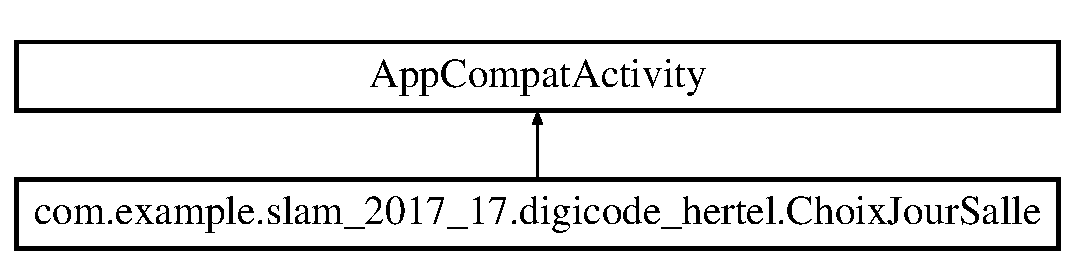
\includegraphics[height=2.000000cm]{classcom_1_1example_1_1slam__2017__17_1_1digicode__hertel_1_1_choix_jour_salle}
\end{center}
\end{figure}
\subsection*{Fonctions membres protégées}
\begin{DoxyCompactItemize}
\item 
void \hyperlink{classcom_1_1example_1_1slam__2017__17_1_1digicode__hertel_1_1_choix_jour_salle_a6d0887f1fed1de0ba657629c0cf181c5}{on\+Create} (Bundle saved\+Instance\+State)
\end{DoxyCompactItemize}


\subsection{Description détaillée}


Définition à la ligne 14 du fichier Choix\+Jour\+Salle.\+java.



\subsection{Documentation des fonctions membres}
\hypertarget{classcom_1_1example_1_1slam__2017__17_1_1digicode__hertel_1_1_choix_jour_salle_a6d0887f1fed1de0ba657629c0cf181c5}{}\index{com\+::example\+::slam\+\_\+2017\+\_\+17\+::digicode\+\_\+hertel\+::\+Choix\+Jour\+Salle@{com\+::example\+::slam\+\_\+2017\+\_\+17\+::digicode\+\_\+hertel\+::\+Choix\+Jour\+Salle}!on\+Create@{on\+Create}}
\index{on\+Create@{on\+Create}!com\+::example\+::slam\+\_\+2017\+\_\+17\+::digicode\+\_\+hertel\+::\+Choix\+Jour\+Salle@{com\+::example\+::slam\+\_\+2017\+\_\+17\+::digicode\+\_\+hertel\+::\+Choix\+Jour\+Salle}}
\subsubsection[{on\+Create(\+Bundle saved\+Instance\+State)}]{\setlength{\rightskip}{0pt plus 5cm}void com.\+example.\+slam\+\_\+2017\+\_\+17.\+digicode\+\_\+hertel.\+Choix\+Jour\+Salle.\+on\+Create (
\begin{DoxyParamCaption}
\item[{Bundle}]{saved\+Instance\+State}
\end{DoxyParamCaption}
)\hspace{0.3cm}{\ttfamily [protected]}}\label{classcom_1_1example_1_1slam__2017__17_1_1digicode__hertel_1_1_choix_jour_salle_a6d0887f1fed1de0ba657629c0cf181c5}
Tableau des salles 

Définition à la ligne 23 du fichier Choix\+Jour\+Salle.\+java.



La documentation de cette classe a été générée à partir du fichier suivant \+:\begin{DoxyCompactItemize}
\item 
java/com/example/slam\+\_\+2017\+\_\+17/digicode\+\_\+hertel/\hyperlink{_choix_jour_salle_8java}{Choix\+Jour\+Salle.\+java}\end{DoxyCompactItemize}

\hypertarget{classcom_1_1example_1_1slam__2017__17_1_1digicode__hertel_1_1_data_base_helper}{}\section{Référence de la classe com.\+example.\+slam\+\_\+2017\+\_\+17.\+digicode\+\_\+hertel.\+Data\+Base\+Helper}
\label{classcom_1_1example_1_1slam__2017__17_1_1digicode__hertel_1_1_data_base_helper}\index{com.\+example.\+slam\+\_\+2017\+\_\+17.\+digicode\+\_\+hertel.\+Data\+Base\+Helper@{com.\+example.\+slam\+\_\+2017\+\_\+17.\+digicode\+\_\+hertel.\+Data\+Base\+Helper}}
Graphe d\textquotesingle{}héritage de com.\+example.\+slam\+\_\+2017\+\_\+17.\+digicode\+\_\+hertel.\+Data\+Base\+Helper\+:\begin{figure}[H]
\begin{center}
\leavevmode
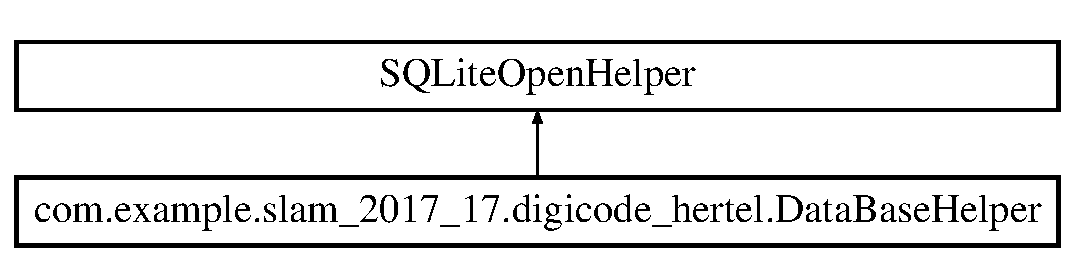
\includegraphics[height=2.000000cm]{classcom_1_1example_1_1slam__2017__17_1_1digicode__hertel_1_1_data_base_helper}
\end{center}
\end{figure}
\subsection*{Fonctions membres publiques}
\begin{DoxyCompactItemize}
\item 
\hyperlink{classcom_1_1example_1_1slam__2017__17_1_1digicode__hertel_1_1_data_base_helper_aa76474b180d0e7768eb06c2aca5a248f}{Data\+Base\+Helper} (Context context)
\item 
void \hyperlink{classcom_1_1example_1_1slam__2017__17_1_1digicode__hertel_1_1_data_base_helper_a656ab8a7805419414c90ea2b9eeb8900}{create\+Data\+Base} ()  throws I\+O\+Exception 
\item 
void \hyperlink{classcom_1_1example_1_1slam__2017__17_1_1digicode__hertel_1_1_data_base_helper_a6467f9cd8cc5811f53fb16d41ca7d17d}{open\+Data\+Base} ()  throws S\+Q\+L\+Exception 
\item 
synchronized void \hyperlink{classcom_1_1example_1_1slam__2017__17_1_1digicode__hertel_1_1_data_base_helper_a9ff7a57fb91953565e199d3e9a106a26}{close} ()
\item 
void \hyperlink{classcom_1_1example_1_1slam__2017__17_1_1digicode__hertel_1_1_data_base_helper_ac5e2fed16a8cb6b58b2768d76f8e324b}{on\+Create} (S\+Q\+Lite\+Database db)
\item 
void \hyperlink{classcom_1_1example_1_1slam__2017__17_1_1digicode__hertel_1_1_data_base_helper_a73dd312883a54c1303ed2da7c2b0c3ca}{on\+Upgrade} (S\+Q\+Lite\+Database db, int old\+Version, int new\+Version)
\item 
boolean \hyperlink{classcom_1_1example_1_1slam__2017__17_1_1digicode__hertel_1_1_data_base_helper_a818c178234e3dc3fb763445813f65153}{login} (String login, String password)
\item 
String \hyperlink{classcom_1_1example_1_1slam__2017__17_1_1digicode__hertel_1_1_data_base_helper_a46c4117ccf1619dfe442ddf270e56c0d}{recup\+Digicode} (Integer jour, Integer salle)
\item 
String\mbox{[}$\,$\mbox{]} \hyperlink{classcom_1_1example_1_1slam__2017__17_1_1digicode__hertel_1_1_data_base_helper_af2239ca86b047c247925472348ab22a2}{recup\+Salles} ()
\end{DoxyCompactItemize}


\subsection{Description détaillée}
Created by slam-\/2017-\/17 on 21/04/2017. 

Définition à la ligne 19 du fichier Data\+Base\+Helper.\+java.



\subsection{Documentation des constructeurs et destructeur}
\hypertarget{classcom_1_1example_1_1slam__2017__17_1_1digicode__hertel_1_1_data_base_helper_aa76474b180d0e7768eb06c2aca5a248f}{}\index{com\+::example\+::slam\+\_\+2017\+\_\+17\+::digicode\+\_\+hertel\+::\+Data\+Base\+Helper@{com\+::example\+::slam\+\_\+2017\+\_\+17\+::digicode\+\_\+hertel\+::\+Data\+Base\+Helper}!Data\+Base\+Helper@{Data\+Base\+Helper}}
\index{Data\+Base\+Helper@{Data\+Base\+Helper}!com\+::example\+::slam\+\_\+2017\+\_\+17\+::digicode\+\_\+hertel\+::\+Data\+Base\+Helper@{com\+::example\+::slam\+\_\+2017\+\_\+17\+::digicode\+\_\+hertel\+::\+Data\+Base\+Helper}}
\subsubsection[{Data\+Base\+Helper(\+Context context)}]{\setlength{\rightskip}{0pt plus 5cm}com.\+example.\+slam\+\_\+2017\+\_\+17.\+digicode\+\_\+hertel.\+Data\+Base\+Helper.\+Data\+Base\+Helper (
\begin{DoxyParamCaption}
\item[{Context}]{context}
\end{DoxyParamCaption}
)}\label{classcom_1_1example_1_1slam__2017__17_1_1digicode__hertel_1_1_data_base_helper_aa76474b180d0e7768eb06c2aca5a248f}
Constructor Takes and keeps a reference of the passed context in order to access to the application assets and resources. 
\begin{DoxyParams}{Paramètres}
{\em context} & \\
\hline
\end{DoxyParams}


Définition à la ligne 34 du fichier Data\+Base\+Helper.\+java.



\subsection{Documentation des fonctions membres}
\hypertarget{classcom_1_1example_1_1slam__2017__17_1_1digicode__hertel_1_1_data_base_helper_a9ff7a57fb91953565e199d3e9a106a26}{}\index{com\+::example\+::slam\+\_\+2017\+\_\+17\+::digicode\+\_\+hertel\+::\+Data\+Base\+Helper@{com\+::example\+::slam\+\_\+2017\+\_\+17\+::digicode\+\_\+hertel\+::\+Data\+Base\+Helper}!close@{close}}
\index{close@{close}!com\+::example\+::slam\+\_\+2017\+\_\+17\+::digicode\+\_\+hertel\+::\+Data\+Base\+Helper@{com\+::example\+::slam\+\_\+2017\+\_\+17\+::digicode\+\_\+hertel\+::\+Data\+Base\+Helper}}
\subsubsection[{close()}]{\setlength{\rightskip}{0pt plus 5cm}synchronized void com.\+example.\+slam\+\_\+2017\+\_\+17.\+digicode\+\_\+hertel.\+Data\+Base\+Helper.\+close (
\begin{DoxyParamCaption}
{}
\end{DoxyParamCaption}
)}\label{classcom_1_1example_1_1slam__2017__17_1_1digicode__hertel_1_1_data_base_helper_a9ff7a57fb91953565e199d3e9a106a26}


Définition à la ligne 137 du fichier Data\+Base\+Helper.\+java.

\hypertarget{classcom_1_1example_1_1slam__2017__17_1_1digicode__hertel_1_1_data_base_helper_a656ab8a7805419414c90ea2b9eeb8900}{}\index{com\+::example\+::slam\+\_\+2017\+\_\+17\+::digicode\+\_\+hertel\+::\+Data\+Base\+Helper@{com\+::example\+::slam\+\_\+2017\+\_\+17\+::digicode\+\_\+hertel\+::\+Data\+Base\+Helper}!create\+Data\+Base@{create\+Data\+Base}}
\index{create\+Data\+Base@{create\+Data\+Base}!com\+::example\+::slam\+\_\+2017\+\_\+17\+::digicode\+\_\+hertel\+::\+Data\+Base\+Helper@{com\+::example\+::slam\+\_\+2017\+\_\+17\+::digicode\+\_\+hertel\+::\+Data\+Base\+Helper}}
\subsubsection[{create\+Data\+Base()}]{\setlength{\rightskip}{0pt plus 5cm}void com.\+example.\+slam\+\_\+2017\+\_\+17.\+digicode\+\_\+hertel.\+Data\+Base\+Helper.\+create\+Data\+Base (
\begin{DoxyParamCaption}
{}
\end{DoxyParamCaption}
) throws I\+O\+Exception}\label{classcom_1_1example_1_1slam__2017__17_1_1digicode__hertel_1_1_data_base_helper_a656ab8a7805419414c90ea2b9eeb8900}
Creates a empty database on the system and rewrites it with your own database. 

Définition à la ligne 43 du fichier Data\+Base\+Helper.\+java.

\hypertarget{classcom_1_1example_1_1slam__2017__17_1_1digicode__hertel_1_1_data_base_helper_a818c178234e3dc3fb763445813f65153}{}\index{com\+::example\+::slam\+\_\+2017\+\_\+17\+::digicode\+\_\+hertel\+::\+Data\+Base\+Helper@{com\+::example\+::slam\+\_\+2017\+\_\+17\+::digicode\+\_\+hertel\+::\+Data\+Base\+Helper}!login@{login}}
\index{login@{login}!com\+::example\+::slam\+\_\+2017\+\_\+17\+::digicode\+\_\+hertel\+::\+Data\+Base\+Helper@{com\+::example\+::slam\+\_\+2017\+\_\+17\+::digicode\+\_\+hertel\+::\+Data\+Base\+Helper}}
\subsubsection[{login(\+String login, String password)}]{\setlength{\rightskip}{0pt plus 5cm}boolean com.\+example.\+slam\+\_\+2017\+\_\+17.\+digicode\+\_\+hertel.\+Data\+Base\+Helper.\+login (
\begin{DoxyParamCaption}
\item[{String}]{login, }
\item[{String}]{password}
\end{DoxyParamCaption}
)}\label{classcom_1_1example_1_1slam__2017__17_1_1digicode__hertel_1_1_data_base_helper_a818c178234e3dc3fb763445813f65153}


Définition à la ligne 161 du fichier Data\+Base\+Helper.\+java.

\hypertarget{classcom_1_1example_1_1slam__2017__17_1_1digicode__hertel_1_1_data_base_helper_ac5e2fed16a8cb6b58b2768d76f8e324b}{}\index{com\+::example\+::slam\+\_\+2017\+\_\+17\+::digicode\+\_\+hertel\+::\+Data\+Base\+Helper@{com\+::example\+::slam\+\_\+2017\+\_\+17\+::digicode\+\_\+hertel\+::\+Data\+Base\+Helper}!on\+Create@{on\+Create}}
\index{on\+Create@{on\+Create}!com\+::example\+::slam\+\_\+2017\+\_\+17\+::digicode\+\_\+hertel\+::\+Data\+Base\+Helper@{com\+::example\+::slam\+\_\+2017\+\_\+17\+::digicode\+\_\+hertel\+::\+Data\+Base\+Helper}}
\subsubsection[{on\+Create(\+S\+Q\+Lite\+Database db)}]{\setlength{\rightskip}{0pt plus 5cm}void com.\+example.\+slam\+\_\+2017\+\_\+17.\+digicode\+\_\+hertel.\+Data\+Base\+Helper.\+on\+Create (
\begin{DoxyParamCaption}
\item[{S\+Q\+Lite\+Database}]{db}
\end{DoxyParamCaption}
)}\label{classcom_1_1example_1_1slam__2017__17_1_1digicode__hertel_1_1_data_base_helper_ac5e2fed16a8cb6b58b2768d76f8e324b}


Définition à la ligne 147 du fichier Data\+Base\+Helper.\+java.

\hypertarget{classcom_1_1example_1_1slam__2017__17_1_1digicode__hertel_1_1_data_base_helper_a73dd312883a54c1303ed2da7c2b0c3ca}{}\index{com\+::example\+::slam\+\_\+2017\+\_\+17\+::digicode\+\_\+hertel\+::\+Data\+Base\+Helper@{com\+::example\+::slam\+\_\+2017\+\_\+17\+::digicode\+\_\+hertel\+::\+Data\+Base\+Helper}!on\+Upgrade@{on\+Upgrade}}
\index{on\+Upgrade@{on\+Upgrade}!com\+::example\+::slam\+\_\+2017\+\_\+17\+::digicode\+\_\+hertel\+::\+Data\+Base\+Helper@{com\+::example\+::slam\+\_\+2017\+\_\+17\+::digicode\+\_\+hertel\+::\+Data\+Base\+Helper}}
\subsubsection[{on\+Upgrade(\+S\+Q\+Lite\+Database db, int old\+Version, int new\+Version)}]{\setlength{\rightskip}{0pt plus 5cm}void com.\+example.\+slam\+\_\+2017\+\_\+17.\+digicode\+\_\+hertel.\+Data\+Base\+Helper.\+on\+Upgrade (
\begin{DoxyParamCaption}
\item[{S\+Q\+Lite\+Database}]{db, }
\item[{int}]{old\+Version, }
\item[{int}]{new\+Version}
\end{DoxyParamCaption}
)}\label{classcom_1_1example_1_1slam__2017__17_1_1digicode__hertel_1_1_data_base_helper_a73dd312883a54c1303ed2da7c2b0c3ca}


Définition à la ligne 152 du fichier Data\+Base\+Helper.\+java.

\hypertarget{classcom_1_1example_1_1slam__2017__17_1_1digicode__hertel_1_1_data_base_helper_a6467f9cd8cc5811f53fb16d41ca7d17d}{}\index{com\+::example\+::slam\+\_\+2017\+\_\+17\+::digicode\+\_\+hertel\+::\+Data\+Base\+Helper@{com\+::example\+::slam\+\_\+2017\+\_\+17\+::digicode\+\_\+hertel\+::\+Data\+Base\+Helper}!open\+Data\+Base@{open\+Data\+Base}}
\index{open\+Data\+Base@{open\+Data\+Base}!com\+::example\+::slam\+\_\+2017\+\_\+17\+::digicode\+\_\+hertel\+::\+Data\+Base\+Helper@{com\+::example\+::slam\+\_\+2017\+\_\+17\+::digicode\+\_\+hertel\+::\+Data\+Base\+Helper}}
\subsubsection[{open\+Data\+Base()}]{\setlength{\rightskip}{0pt plus 5cm}void com.\+example.\+slam\+\_\+2017\+\_\+17.\+digicode\+\_\+hertel.\+Data\+Base\+Helper.\+open\+Data\+Base (
\begin{DoxyParamCaption}
{}
\end{DoxyParamCaption}
) throws S\+Q\+L\+Exception}\label{classcom_1_1example_1_1slam__2017__17_1_1digicode__hertel_1_1_data_base_helper_a6467f9cd8cc5811f53fb16d41ca7d17d}


Définition à la ligne 128 du fichier Data\+Base\+Helper.\+java.

\hypertarget{classcom_1_1example_1_1slam__2017__17_1_1digicode__hertel_1_1_data_base_helper_a46c4117ccf1619dfe442ddf270e56c0d}{}\index{com\+::example\+::slam\+\_\+2017\+\_\+17\+::digicode\+\_\+hertel\+::\+Data\+Base\+Helper@{com\+::example\+::slam\+\_\+2017\+\_\+17\+::digicode\+\_\+hertel\+::\+Data\+Base\+Helper}!recup\+Digicode@{recup\+Digicode}}
\index{recup\+Digicode@{recup\+Digicode}!com\+::example\+::slam\+\_\+2017\+\_\+17\+::digicode\+\_\+hertel\+::\+Data\+Base\+Helper@{com\+::example\+::slam\+\_\+2017\+\_\+17\+::digicode\+\_\+hertel\+::\+Data\+Base\+Helper}}
\subsubsection[{recup\+Digicode(\+Integer jour, Integer salle)}]{\setlength{\rightskip}{0pt plus 5cm}String com.\+example.\+slam\+\_\+2017\+\_\+17.\+digicode\+\_\+hertel.\+Data\+Base\+Helper.\+recup\+Digicode (
\begin{DoxyParamCaption}
\item[{Integer}]{jour, }
\item[{Integer}]{salle}
\end{DoxyParamCaption}
)}\label{classcom_1_1example_1_1slam__2017__17_1_1digicode__hertel_1_1_data_base_helper_a46c4117ccf1619dfe442ddf270e56c0d}


Définition à la ligne 183 du fichier Data\+Base\+Helper.\+java.

\hypertarget{classcom_1_1example_1_1slam__2017__17_1_1digicode__hertel_1_1_data_base_helper_af2239ca86b047c247925472348ab22a2}{}\index{com\+::example\+::slam\+\_\+2017\+\_\+17\+::digicode\+\_\+hertel\+::\+Data\+Base\+Helper@{com\+::example\+::slam\+\_\+2017\+\_\+17\+::digicode\+\_\+hertel\+::\+Data\+Base\+Helper}!recup\+Salles@{recup\+Salles}}
\index{recup\+Salles@{recup\+Salles}!com\+::example\+::slam\+\_\+2017\+\_\+17\+::digicode\+\_\+hertel\+::\+Data\+Base\+Helper@{com\+::example\+::slam\+\_\+2017\+\_\+17\+::digicode\+\_\+hertel\+::\+Data\+Base\+Helper}}
\subsubsection[{recup\+Salles()}]{\setlength{\rightskip}{0pt plus 5cm}String \mbox{[}$\,$\mbox{]} com.\+example.\+slam\+\_\+2017\+\_\+17.\+digicode\+\_\+hertel.\+Data\+Base\+Helper.\+recup\+Salles (
\begin{DoxyParamCaption}
{}
\end{DoxyParamCaption}
)}\label{classcom_1_1example_1_1slam__2017__17_1_1digicode__hertel_1_1_data_base_helper_af2239ca86b047c247925472348ab22a2}


Définition à la ligne 195 du fichier Data\+Base\+Helper.\+java.



La documentation de cette classe a été générée à partir du fichier suivant \+:\begin{DoxyCompactItemize}
\item 
java/com/example/slam\+\_\+2017\+\_\+17/digicode\+\_\+hertel/\hyperlink{_data_base_helper_8java}{Data\+Base\+Helper.\+java}\end{DoxyCompactItemize}

\hypertarget{classcom_1_1example_1_1slam__2017__17_1_1digicode__hertel_1_1_main_activity}{}\section{Référence de la classe com.\+example.\+slam\+\_\+2017\+\_\+17.\+digicode\+\_\+hertel.\+Main\+Activity}
\label{classcom_1_1example_1_1slam__2017__17_1_1digicode__hertel_1_1_main_activity}\index{com.\+example.\+slam\+\_\+2017\+\_\+17.\+digicode\+\_\+hertel.\+Main\+Activity@{com.\+example.\+slam\+\_\+2017\+\_\+17.\+digicode\+\_\+hertel.\+Main\+Activity}}
Graphe d\textquotesingle{}héritage de com.\+example.\+slam\+\_\+2017\+\_\+17.\+digicode\+\_\+hertel.\+Main\+Activity\+:\begin{figure}[H]
\begin{center}
\leavevmode
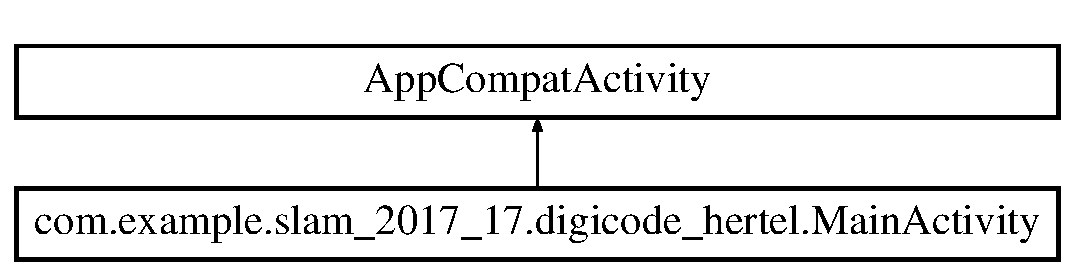
\includegraphics[height=2.000000cm]{classcom_1_1example_1_1slam__2017__17_1_1digicode__hertel_1_1_main_activity}
\end{center}
\end{figure}
\subsection*{Fonctions membres protégées}
\begin{DoxyCompactItemize}
\item 
void \hyperlink{classcom_1_1example_1_1slam__2017__17_1_1digicode__hertel_1_1_main_activity_ac28f62bda94de44539157879a4a422e8}{on\+Create} (Bundle saved\+Instance\+State)
\end{DoxyCompactItemize}


\subsection{Description détaillée}


Définition à la ligne 11 du fichier Main\+Activity.\+java.



\subsection{Documentation des fonctions membres}
\hypertarget{classcom_1_1example_1_1slam__2017__17_1_1digicode__hertel_1_1_main_activity_ac28f62bda94de44539157879a4a422e8}{}\index{com\+::example\+::slam\+\_\+2017\+\_\+17\+::digicode\+\_\+hertel\+::\+Main\+Activity@{com\+::example\+::slam\+\_\+2017\+\_\+17\+::digicode\+\_\+hertel\+::\+Main\+Activity}!on\+Create@{on\+Create}}
\index{on\+Create@{on\+Create}!com\+::example\+::slam\+\_\+2017\+\_\+17\+::digicode\+\_\+hertel\+::\+Main\+Activity@{com\+::example\+::slam\+\_\+2017\+\_\+17\+::digicode\+\_\+hertel\+::\+Main\+Activity}}
\subsubsection[{on\+Create(\+Bundle saved\+Instance\+State)}]{\setlength{\rightskip}{0pt plus 5cm}void com.\+example.\+slam\+\_\+2017\+\_\+17.\+digicode\+\_\+hertel.\+Main\+Activity.\+on\+Create (
\begin{DoxyParamCaption}
\item[{Bundle}]{saved\+Instance\+State}
\end{DoxyParamCaption}
)\hspace{0.3cm}{\ttfamily [protected]}}\label{classcom_1_1example_1_1slam__2017__17_1_1digicode__hertel_1_1_main_activity_ac28f62bda94de44539157879a4a422e8}


Définition à la ligne 19 du fichier Main\+Activity.\+java.



La documentation de cette classe a été générée à partir du fichier suivant \+:\begin{DoxyCompactItemize}
\item 
java/com/example/slam\+\_\+2017\+\_\+17/digicode\+\_\+hertel/\hyperlink{_main_activity_8java}{Main\+Activity.\+java}\end{DoxyCompactItemize}

\chapter{Documentation des fichiers}
\hypertarget{_choix_date_salle_8java}{}\section{Référence du fichier java/com/example/slam\+\_\+2017\+\_\+17/digicode\+\_\+hertel/\+Choix\+Date\+Salle.java}
\label{_choix_date_salle_8java}\index{java/com/example/slam\+\_\+2017\+\_\+17/digicode\+\_\+hertel/\+Choix\+Date\+Salle.\+java@{java/com/example/slam\+\_\+2017\+\_\+17/digicode\+\_\+hertel/\+Choix\+Date\+Salle.\+java}}
\subsection*{Classes}
\begin{DoxyCompactItemize}
\item 
class \hyperlink{classcom_1_1example_1_1slam__2017__17_1_1digicode__hertel_1_1_choix_date_salle}{com.\+example.\+slam\+\_\+2017\+\_\+17.\+digicode\+\_\+hertel.\+Choix\+Date\+Salle}
\end{DoxyCompactItemize}
\subsection*{Paquetages}
\begin{DoxyCompactItemize}
\item 
package \hyperlink{namespacecom_1_1example_1_1slam__2017__17_1_1digicode__hertel}{com.\+example.\+slam\+\_\+2017\+\_\+17.\+digicode\+\_\+hertel}
\end{DoxyCompactItemize}

\hypertarget{_choix_jour_salle_8java}{}\section{Référence du fichier java/com/example/slam\+\_\+2017\+\_\+17/digicode\+\_\+hertel/\+Choix\+Jour\+Salle.java}
\label{_choix_jour_salle_8java}\index{java/com/example/slam\+\_\+2017\+\_\+17/digicode\+\_\+hertel/\+Choix\+Jour\+Salle.\+java@{java/com/example/slam\+\_\+2017\+\_\+17/digicode\+\_\+hertel/\+Choix\+Jour\+Salle.\+java}}
\subsection*{Classes}
\begin{DoxyCompactItemize}
\item 
class \hyperlink{classcom_1_1example_1_1slam__2017__17_1_1digicode__hertel_1_1_choix_jour_salle}{com.\+example.\+slam\+\_\+2017\+\_\+17.\+digicode\+\_\+hertel.\+Choix\+Jour\+Salle}
\end{DoxyCompactItemize}
\subsection*{Paquetages}
\begin{DoxyCompactItemize}
\item 
package \hyperlink{namespacecom_1_1example_1_1slam__2017__17_1_1digicode__hertel}{com.\+example.\+slam\+\_\+2017\+\_\+17.\+digicode\+\_\+hertel}
\end{DoxyCompactItemize}

\hypertarget{_data_base_helper_8java}{}\section{Référence du fichier java/com/example/slam\+\_\+2017\+\_\+17/digicode\+\_\+hertel/\+Data\+Base\+Helper.java}
\label{_data_base_helper_8java}\index{java/com/example/slam\+\_\+2017\+\_\+17/digicode\+\_\+hertel/\+Data\+Base\+Helper.\+java@{java/com/example/slam\+\_\+2017\+\_\+17/digicode\+\_\+hertel/\+Data\+Base\+Helper.\+java}}
\subsection*{Classes}
\begin{DoxyCompactItemize}
\item 
class \hyperlink{classcom_1_1example_1_1slam__2017__17_1_1digicode__hertel_1_1_data_base_helper}{com.\+example.\+slam\+\_\+2017\+\_\+17.\+digicode\+\_\+hertel.\+Data\+Base\+Helper}
\end{DoxyCompactItemize}
\subsection*{Paquetages}
\begin{DoxyCompactItemize}
\item 
package \hyperlink{namespacecom_1_1example_1_1slam__2017__17_1_1digicode__hertel}{com.\+example.\+slam\+\_\+2017\+\_\+17.\+digicode\+\_\+hertel}
\end{DoxyCompactItemize}

\hypertarget{_main_activity_8java}{}\section{Référence du fichier java/com/example/slam\+\_\+2017\+\_\+17/digicode\+\_\+hertel/\+Main\+Activity.java}
\label{_main_activity_8java}\index{java/com/example/slam\+\_\+2017\+\_\+17/digicode\+\_\+hertel/\+Main\+Activity.\+java@{java/com/example/slam\+\_\+2017\+\_\+17/digicode\+\_\+hertel/\+Main\+Activity.\+java}}
\subsection*{Classes}
\begin{DoxyCompactItemize}
\item 
class \hyperlink{classcom_1_1example_1_1slam__2017__17_1_1digicode__hertel_1_1_main_activity}{com.\+example.\+slam\+\_\+2017\+\_\+17.\+digicode\+\_\+hertel.\+Main\+Activity}
\end{DoxyCompactItemize}
\subsection*{Paquetages}
\begin{DoxyCompactItemize}
\item 
package \hyperlink{namespacecom_1_1example_1_1slam__2017__17_1_1digicode__hertel}{com.\+example.\+slam\+\_\+2017\+\_\+17.\+digicode\+\_\+hertel}
\end{DoxyCompactItemize}

%--- End generated contents ---

% Index
\backmatter
\newpage
\phantomsection
\clearemptydoublepage
\addcontentsline{toc}{chapter}{Index}
\printindex

\end{document}
